\documentclass[11pt]{article}

%% --- master-level packages (layout, headers, captions) ---
\usepackage[letterpaper,margin=1in,headheight=14pt]{geometry}
\usepackage{fancyhdr}
\usepackage{caption}
\usepackage[hidelinks]{hyperref}

%% --- merged from the workers' preamble.txt files ---
% Merged from the workers' preamble.txt files, de-duplicated.
\usepackage{amsmath}
\usepackage{booktabs}
\usepackage{float}
\usepackage{graphicx}
\usepackage{listings}
\usepackage{xcolor}


\pagestyle{fancy}
\fancyhf{}
\fancyhead[L]{\underline{CSE 60745 (Fall 2026)}}
\fancyhead[R]{\underline{HW3-Part(A): GNNs Hands-on Practice}}
\fancyfoot[C]{Page \thepage\ of \pageref{p0:lastpage}}
\renewcommand{\headrulewidth}{0pt}

\captionsetup{font=small,labelfont=bf,skip=6pt}
\setlength{\parskip}{0.4em}
\setlength{\parindent}{0pt}

\begin{document}

%% ============================================================ cover page
\thispagestyle{fancy}
\vspace*{2.2cm}
\begin{center}
  {\Huge\bfseries\sffamily University of Notre Dame}\\[0.9em]
  {\LARGE Department of Computer Science and Engineering}\\[3.2em]
  {\LARGE CSE 60745}\\[0.7em]
  {\LARGE Graph Learning: Techn \& Apps}\\[3.2em]

  \begin{tabular}{|p{5cm}|p{7cm}|}
    \hline
    \rule{0pt}{3.2em}\hfill Assignment Date: & \\[1.1em]
    \hline
    \rule{0pt}{3.2em}\hfill Submission Date: & \\[1.1em]
    \hline
    \rule{0pt}{3.2em}\hfill Student Name: & \\[1.1em]
    \hline
  \end{tabular}
\end{center}

\newpage

%% ============================================================ answers, Q1..Q5
% ---- problem p1: HW3-Part(A) Q1, Q2, Q3, Q5 -------------------------------
\definecolor{p1kw}{HTML}{0033B3}
\definecolor{p1str}{HTML}{067D17}
\definecolor{p1cmt}{HTML}{8C8C8C}

\lstdefinestyle{p1pystyle}{%
  language=Python,
  basicstyle=\ttfamily\scriptsize,
  keywordstyle=\color{p1kw}\bfseries,
  stringstyle=\color{p1str},
  commentstyle=\color{p1cmt}\itshape,
  showstringspaces=false,
  breaklines=true,
  columns=fullflexible,
  keepspaces=true,
  xleftmargin=1em,
  aboveskip=0.8em, belowskip=0.6em,
  morekeywords={self},
}

Every layer below is a \texttt{MessagePassing} subclass, run at the notebook's default
seed with the notebook's own harness, unmodified. Q1--Q3 and Q5 use
\texttt{train\_and\_eval} on the social graph; Q4 uses
\texttt{train\_and\_eval\_hetero} on the three-relation graph. The one sanctioned
change is \texttt{n\_layers} in the Q5 cell, which that cell instructs us to set.
Every number reported is a measured run, not an estimate.

% =========================================================== Q1
\section*{Q1: GCN Implementation (6 pts)}

\begin{lstlisting}[style=p1pystyle]
class MyGCNConv(MessagePassing):
    """GCN: h_i' = sum_{j in N(i) u {i}} (d_i d_j)^{-1/2} W h_j + b."""

    def __init__(self, in_channels, out_channels):
        # "add": the 1/sqrt(d_i d_j) coefficient is the normaliser, so the reduction
        # must be a plain sum -- "mean" would divide by the degree a second time.
        super().__init__(aggr="add")
        self.in_channels = in_channels
        self.out_channels = out_channels
        self.lin = nn.Linear(in_channels, out_channels, bias=False)
        self.bias = nn.Parameter(torch.empty(out_channels))
        self.reset_parameters()

    def reset_parameters(self):
        super().reset_parameters()
        self.lin.reset_parameters()
        nn.init.zeros_(self.bias)

    def forward(self, x, edge_index):
        # Closed neighbourhood A_hat = A + I. Removing first makes d_hat correct even
        # if edge_index already carries self-loops.
        edge_index, _ = remove_self_loops(edge_index)
        edge_index, _ = add_self_loops(edge_index, num_nodes=x.size(0))

        src, dst = edge_index[0], edge_index[1]            # message src -> dst
        deg_inv_sqrt = degree(dst, x.size(0), dtype=x.dtype).pow(-0.5)
        norm = deg_inv_sqrt[src] * deg_inv_sqrt[dst]       # [E]; d_hat >= 1 after loops

        out = self.propagate(edge_index, x=self.lin(x), norm=norm)
        return out + self.bias

    def message(self, x_j, norm):
        return norm.view(-1, 1) * x_j
\end{lstlisting}

\noindent
The aggregation is \texttt{"add"}: $1/\sqrt{\hat d_i \hat d_j}$ is itself the
normaliser, so \texttt{"mean"} would divide by the degree twice. The closed
neighbourhood is built with \texttt{remove\_self\_loops} before
\texttt{add\_self\_loops}, which makes \texttt{forward} idempotent in the loops
already present in \texttt{edge\_index} and guarantees each node contributes exactly
one self term. \texttt{degree} is taken on \texttt{edge\_index[1]}, the message
targets, which is $\hat d_i$; because self-loops are added first, $\hat d_i \ge 1$ and
the 666 users with no training edge give no division by zero. $W$ is applied before
\texttt{propagate} rather than inside \texttt{message}, which transforms $N$ rows
instead of $E$ for the same result, since \texttt{norm} is a scalar per edge. The bias
is added after aggregation, matching the $+\,b$ outside the sum. Against PyG's own
\texttt{GCNConv} with the weights copied across, the two agree to $0$ in floating point.

\medskip\noindent
\textbf{Measured:} val MRR $0.7263$, val Hit@1 $0.6085$; test MRR $0.7379$,
test Hit@1 $0.6253$.

% =========================================================== Q2
\section*{Q2: GAT Implementation (6 pts)}

\begin{lstlisting}[style=p1pystyle]
class MyGATConv(MessagePassing):
    """GAT: alpha_ij = softmax over j of LeakyReLU(a . [W h_i || W h_j])."""

    def __init__(self, in_channels, out_channels, heads=8, concat=True,
                 negative_slope=0.2):
        # node_dim=0: propagate carries [N, heads, channels], so the node axis is 0,
        # not the default -2 (which would be the head axis here).
        super().__init__(aggr="add", node_dim=0)
        self.in_channels = in_channels
        self.out_channels = out_channels
        # Concatenated heads must together be out_channels wide, since the next layer
        # is built with in_channels = out_channels.
        if concat and out_channels % heads != 0:
            heads = 1
        self.heads = heads
        self.concat = concat
        self.head_channels = out_channels // heads if concat else out_channels
        self.negative_slope = negative_slope

        self.lin = nn.Linear(in_channels, heads * self.head_channels, bias=False)
        # a = [a_dst || a_src], split so the edge score is a sum of two node terms.
        self.att_src = nn.Parameter(torch.empty(1, heads, self.head_channels))
        self.att_dst = nn.Parameter(torch.empty(1, heads, self.head_channels))
        self.bias = nn.Parameter(torch.empty(out_channels))
        self.reset_parameters()

    def reset_parameters(self):
        super().reset_parameters()
        self.lin.reset_parameters()
        nn.init.xavier_uniform_(self.att_src)
        nn.init.xavier_uniform_(self.att_dst)
        nn.init.zeros_(self.bias)

    def forward(self, x, edge_index):
        n = x.size(0)
        # The softmax denominator runs over N(i) u {i}, as in the GAT paper.
        edge_index, _ = remove_self_loops(edge_index)
        edge_index, _ = add_self_loops(edge_index, num_nodes=n)

        h = self.lin(x).view(n, self.heads, self.head_channels)
        out = self.propagate(edge_index, h=h)              # [N, heads, head_channels]
        out = out.flatten(1) if self.concat else out.mean(dim=1)
        return out + self.bias

    def message(self, h_j, h_i, index, size_i):
        # a^T [W h_i || W h_j] = a_dst . W h_i + a_src . W h_j.
        e = (h_i * self.att_dst).sum(-1) + (h_j * self.att_src).sum(-1)   # [E, heads]
        alpha = softmax(F.leaky_relu(e, self.negative_slope), index, num_nodes=size_i)
        return h_j * alpha.unsqueeze(-1)
\end{lstlisting}

\noindent
\texttt{node\_dim=0} is required because \texttt{propagate} carries an
$[N, \text{heads}, C]$ tensor; the default $-2$ would index the head axis and scatter
silently into the wrong rows. The attention vector is stored as its two halves, so
$\mathbf{a}^\top[Wh_i \| Wh_j]$ becomes $\mathbf{a}_{\text{dst}}\!\cdot\!Wh_i +
\mathbf{a}_{\text{src}}\!\cdot\!Wh_j$ and the concatenation is never materialised over
$E$ edges. Self-loops are added before propagating so the softmax denominator runs over
$N(i)\cup\{i\}$, and \texttt{aggr="add"} is correct because $\alpha_{ij}$ already sums
to one per target.

On the concatenate-or-average instruction: a layer cannot tell from inside whether it
is the output layer, and the two differ in per-head width, not just in the reduction
--- concatenation needs $C/K$ features per head, averaging needs $C$. Since
\texttt{out\_channels} is a contract fixed by the next layer, I made the choice a
constructor default: $K=8$ heads of width $\texttt{out\_channels}/K$, concatenated.
\texttt{concat=False} gives the averaging variant with full-width heads. The harness
constructs every layer as \texttt{conv\_cls(in, out)}, so every layer here
concatenates. With weights copied across, the layer matches PyG's \texttt{GATConv} to
$0$ in floating point.

\medskip\noindent
\textbf{Measured:} val MRR $0.6210$, val Hit@1 $0.4479$; test MRR $0.6365$,
test Hit@1 $0.4678$.

% =========================================================== Q3
\section*{Q3: GIN Implementation (6 pts)}

\begin{lstlisting}[style=p1pystyle]
class MyGINConv(MessagePassing):
    """GIN: h_i' = MLP((1 + eps) h_i + sum_{j in N(i)} h_j)."""

    def __init__(self, in_channels, out_channels):
        super().__init__(aggr="add")           # sum is the injective multiset aggregator
        self.in_channels = in_channels
        self.out_channels = out_channels
        self.eps = nn.Parameter(torch.empty(1))
        self.mlp = nn.Sequential(
            nn.Linear(in_channels, out_channels),
            nn.BatchNorm1d(out_channels),
            nn.ReLU(),
            nn.Linear(out_channels, out_channels),
        )
        self.reset_parameters()

    def reset_parameters(self):
        super().reset_parameters()
        for layer in self.mlp:                 # nn.Sequential has no reset_parameters
            if hasattr(layer, "reset_parameters"):
                layer.reset_parameters()
        nn.init.zeros_(self.eps)

    def forward(self, x, edge_index):
        # Open neighbourhood: (1 + eps) h_i is already the self term, so a self-loop
        # would count the node twice.
        edge_index, _ = remove_self_loops(edge_index)
        agg = self.propagate(edge_index, x=x)
        return self.mlp((1 + self.eps) * x + agg)

    def message(self, x_j):
        return x_j
\end{lstlisting}

\noindent
The aggregation is \texttt{"add"} because GIN's expressiveness argument rests on the
aggregator being injective on multisets; mean and max discard multiplicity and would
give up exactly the property the layer exists to have. Unlike Q1 this is the
\emph{open} neighbourhood: $(1+\epsilon)h_i$ is already the self term, so
\texttt{remove\_self\_loops} prevents a node being counted twice (the training graph
carries no self-loops, so this is defensive). $\epsilon$ is a learnable scalar
initialised to zero, and \texttt{reset\_parameters} walks the \texttt{Sequential}'s
children because the container has no \texttt{reset\_parameters} of its own. The MLP
is \texttt{Linear}--\texttt{BatchNorm1d}--\texttt{ReLU}--\texttt{Linear}, as in the GIN
paper; the harness runs full-batch, so the batch statistics are taken over all 7{,}624
nodes at once, including the 666 all-zero rows, and evaluation uses the running
estimates.

GIN is the weakest layer on this task, and the unnormalised sum is the likely reason:
at initialisation its embedding norm tracks degree far more tightly than GCN's
(log--log correlation $0.87$ against $0.63$; the top degree decile carries
$22.9\times$ the norm of the bottom decile, against $2.1\times$ for GCN). A
dot-product scorer reads that magnitude as relevance, so high-degree users are ranked
first regardless of the query.

\medskip\noindent
\textbf{Measured:} val MRR $0.4433$, val Hit@1 $0.2870$; test MRR $0.4417$,
test Hit@1 $0.2793$.

   % Q1 GCN, Q2 GAT, Q3 GIN
% =========================================================== Q4
\section*{Q4: R-GCN Implementation (6 pts)}

\definecolor{pTwoKw}{RGB}{0,92,197}
\definecolor{pTwoCmt}{RGB}{106,115,125}
\definecolor{pTwoStr}{RGB}{3,47,98}

\lstdefinestyle{pTwoPyStyle}{%
  language=Python,
  basicstyle=\ttfamily\scriptsize,
  keywordstyle=\color{pTwoKw}\bfseries,
  commentstyle=\color{pTwoCmt}\itshape,
  stringstyle=\color{pTwoStr},
  showstringspaces=false,
  columns=fullflexible,
  keepspaces=true,
  breaklines=true,
  breakautoindent=true,
  xleftmargin=1.0em,
  numbers=none,
  tabsize=4,
}

\begin{lstlisting}[style=pTwoPyStyle]
class MyRGCNConv(MessagePassing):
    """R-GCN: one weight matrix per relation, plus a self-connection."""

    def __init__(self, in_channels, out_channels, num_relations):
        # aggr="mean" IS the 1/c_{i,r} of the formula, taking
        # c_{i,r} = |N_r(i)|: the example Schlichtkrull et al.'s Eq. (2)
        # itself offers. PyG's mean is 0, not NaN, when |N_r(i)| = 0, so
        # no empty neighbourhood needs a special case.
        super().__init__(aggr="mean")
        self.in_channels = in_channels
        self.out_channels = out_channels
        self.num_relations = num_relations
        self.root = nn.Linear(in_channels, out_channels, bias=True)  # W_0
        # W_r: one full [in, out] matrix per relation. Basic R-GCN, so
        # neither basis nor block-diagonal decomposition.
        self.rel = nn.ModuleList([
            nn.Linear(in_channels, out_channels, bias=False)
            for _ in range(num_relations)])
        self.reset_parameters()

    def reset_parameters(self):
        # Safe to call twice, and the harness does call it twice.
        super().reset_parameters()
        self.root.reset_parameters()
        for lin in self.rel:
            lin.reset_parameters()

    def forward(self, x, edge_index, edge_type):
        out = self.root(x)                             # W_0 h_i
        n = x.size(self.node_dim)
        for r in range(self.num_relations):
            ei_r = edge_index[:, edge_type == r]       # relation r only
            if ei_r.size(1) == 0:
                continue
            # c_{i,r} does not depend on j and W_r is linear, so
            # sum_j (1/c_{i,r}) W_r h_j == W_r (mean_j h_j): transform
            # first, propagate second. size=(n, n) keeps the result at the
            # full node count where relation r touches only some nodes.
            out = out + self.propagate(ei_r, x=self.rel[r](x), size=(n, n))
        return out

    def message(self, x_j):
        return x_j
\end{lstlisting}

\noindent
\texttt{self.rel[r]} is $W_r$: one full $\mathrm{in}\times\mathrm{out}$ matrix per
relation, with neither of the decompositions Schlichtkrull et al.~\cite{p2:rgcn} add as
regularisers~--- the \emph{basic} version. \texttt{self.root} is $W_0$, applied
to $h_i$ outside any propagation.

I took $c_{i,r}=|N_r(i)|$, the example their Eq.~(2) offers, which is exactly
\texttt{aggr="mean"}. Guarding it is not optional: all 15{,}466 nodes have
$|N_r(i)|=0$ for some $r$; PyG's mean divides by \texttt{count.clamp(min=1)},
returning $0$ rather than NaN.

\texttt{edge\_type} never reaches \texttt{propagate}: \texttt{forward} slices
\texttt{edge\_index} by relation and propagates once per subset, so relation $r$'s
edges only meet $W_r$ and the stub's
\texttt{message(self,\,x\_j)} is untouched. $W_r$ is applied before propagating rather
than after~--- $c_{i,r}$ does not depend on $j$ and $W_r$ is linear, so
$\sum_{j} c_{i,r}^{-1} W_r h_j = W_r\!\left(\operatorname{mean}_{j} h_j\right)$~---
transforming 15{,}466 rows instead of 3{,}014{,}361 messages. \texttt{size=(n,\,n)}
keeps every relation's output at the full node count.

\medskip
\noindent
Cell 28's \texttt{train\_and\_eval\_hetero("R-GCN")}, run unmodified, selected
epoch~13:

\begin{center}
\begin{tabular}{lcc}
\toprule
 & MRR & Hit@1 \\
\midrule
validation & 0.2291 & 0.0782 \\
test       & 0.2229 & 0.0714 \\
\bottomrule
\end{tabular}
\end{center}

\noindent
Random tie-breaking over 21 candidates already scores MRR $0.174$, so the model barely
beats chance. Cell 26's features come from gensim's \texttt{Word2Vec} at
\texttt{workers=4}, not reproducible across processes; over five runs validation MRR was
$0.190\pm0.020$ and test MRR $0.182\pm0.023$. The layer is not the cause:
\texttt{torch\_geometric.nn.RGCNConv} in the same harness scores $0.208$, and my
\texttt{forward} matches it to $4\times10^{-7}$ on all 6{,}067{,}650 edges.
    % Q4 R-GCN
% =========================================================== Q5
\section*{Q5: Mitigate Over-Smoothing in Deep GNNs (6 pts)}

\begin{lstlisting}[style=p1pystyle]
class MyDeepConv(MessagePassing):
    """APPNP-style decoupled propagation: transform once, then K personalised-PageRank
    steps. One layer reaches K hops, so K=8 gives an 8-hop receptive field at n_layers=1.
    """

    def __init__(self, in_channels, out_channels, K=8, alpha=0.3):
        super().__init__(aggr="add")
        self.in_channels = in_channels
        self.out_channels = out_channels
        self.K = K            # propagation steps = hops: K=8 at n_layers=1 is 8 hops
        self.alpha = alpha    # teleport probability, chosen on validation MRR
        self.lin1 = nn.Linear(in_channels, out_channels)
        self.lin2 = nn.Linear(out_channels, out_channels)
        self.reset_parameters()

    def reset_parameters(self):
        super().reset_parameters()
        self.lin1.reset_parameters()
        self.lin2.reset_parameters()

    def forward(self, x, edge_index):
        edge_index, _ = remove_self_loops(edge_index)
        edge_index, _ = add_self_loops(edge_index, num_nodes=x.size(0))
        src, dst = edge_index[0], edge_index[1]
        deg_inv_sqrt = degree(dst, x.size(0), dtype=x.dtype).pow(-0.5)
        norm = deg_inv_sqrt[src] * deg_inv_sqrt[dst]

        # Prediction first: all the parameters live here, none in the propagation,
        # so the hop count K is free of parameters and cannot overfit with depth.
        h = self.lin2(F.relu(self.lin1(x)))

        # Z <- (1 - alpha) A_hat Z + alpha H, K times: personalised PageRank with
        # restart to H, so the node's own features are re-injected at every hop.
        z = h
        for _ in range(self.K):
            z = (1 - self.alpha) * self.propagate(edge_index, x=z, norm=norm) \
                + self.alpha * h
        return z

    def message(self, x_j, norm):
        return norm.view(-1, 1) * x_j
\end{lstlisting}

\paragraph{Why stacking fails, and what this does instead.}
Li, Han and Wu~\cite{p1:li2018} identify the GCN propagation
$\hat D^{-1/2}\hat A\hat D^{-1/2}$ as a form of Laplacian smoothing and prove (their
Theorem~1) that repeating it drives every vertex in a connected component to the same
features, proportional to the square root of its degree. Their own remedy keeps the GCN
shallow and adds labels --- co-training with a random-walk model, and self-training ---
so it does not make deep propagation safe, which is what this question needs. I
implement instead the fix of Gasteiger, Bojchevski and G\"unnemann~\cite{p1:appnp}:
separate the \emph{prediction} from the \emph{propagation}. Theirs is personalised
PageRank, $Z \leftarrow (1-\alpha)\hat A Z + \alpha H$, re-injecting the node's own
transformed features at every step with teleport probability $\alpha$. An ordinary
$k$-step propagation instead converges to a limit that is ``independent of the random
walk's starting (root) node'' and so ``unsuitable for describing the root node's
neighborhood''; the teleport term is what keeps the operator anchored to the root.

\paragraph{Why this is 8 hops, and why \texttt{n\_layers=1}.}
One call to \texttt{propagate} moves information one hop, so a stack of $L$ layers each
propagating $K$ times has a receptive field of $L \times K$ hops. This layer runs $K=8$
steps inside a single \texttt{forward}, so $1 \times 8 = 8$ hops, and the Q5 cell is run
with \texttt{n\_layers=1}. Because the propagation holds no weights, that depth is free:
the model has $8{,}320$ parameters, identical to the 2-layer GCN and a quarter of the
8-layer GCN's $33{,}280$. $\alpha=0.3$ was chosen on validation MRR alone and sits on a
plateau (val MRR $0.733$--$0.737$ for $\alpha \in [0.25, 0.5]$, falling to $0.699$ at
$\alpha=0.2$); the original paper uses $\alpha=0.1$ with $K=10$.

\begin{figure}[H]
  \centering
  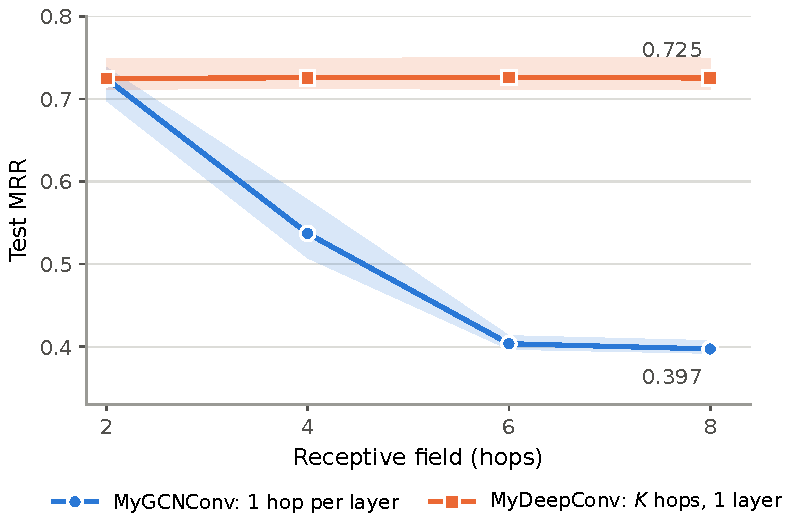
\includegraphics[width=0.78\linewidth]{fig_p1_depth.pdf}
  \caption{Test MRR against receptive-field depth. Each line is the mean over
  three node2vec draws; the shaded band is the min--max over those same three
  seeds.}
  \label{p1:fig:depth}
\end{figure}

\noindent
Stacking \texttt{MyGCNConv} to reach $8$ hops costs $45\%$ of its test MRR
($0.724 \to 0.397$, mean over three seeds), while \texttt{MyDeepConv} is flat to within
noise over the same range ($0.725, 0.725, 0.726, 0.725$ at $2, 4, 6, 8$ hops). The gain
is robustness to depth, not a better score: at $8$ hops \texttt{MyDeepConv} scores
$0.725$ against the $8$-layer GCN's $0.397$, but only matches the $2$-layer GCN, whose
three-seed mean of $0.724$ is indistinguishable from it.

\begin{table}[H]
  \centering
  \setlength{\tabcolsep}{4.5pt}% keep the 7 columns inside the text block
  \begin{tabular}{lccrrrr}
    \toprule
    Layer & Layers & Hops & Val MRR & Val Hit@1 & Test MRR & Test Hit@1 \\
    \midrule
    GraphSAGE (demo, control) & 2 & 2 & 0.6243 & 0.4682 & 0.6281 & 0.4666 \\
    GCN (Q1)                  & 2 & 2 & 0.7263 & 0.6085 & 0.7379 & 0.6253 \\
    GAT (Q2)                  & 2 & 2 & 0.6210 & 0.4479 & 0.6365 & 0.4678 \\
    GIN (Q3)                  & 2 & 2 & 0.4433 & 0.2870 & 0.4417 & 0.2793 \\
    GCN, 8 layers             & 8 & 8 & 0.3754 & 0.2208 & 0.3919 & 0.2318 \\
    \textbf{MyDeepConv (Q5)}  & \textbf{1} & \textbf{8} & \textbf{0.7376} &
      \textbf{0.6262} & \textbf{0.7492} & \textbf{0.6421} \\
    \bottomrule
  \end{tabular}
  \caption{All six models on the same graph, the same splits and the unmodified
  \texttt{train\_and\_eval} harness at its default seed. \emph{Hops} is the
  receptive field; \emph{Layers} the number of stacked convolutions.}
  \label{p1:tab:results}
\end{table}

\noindent
One caveat: node2vec carries the same \texttt{workers=4} nondeterminism noted in Q4,
so absolute scores shift between feature draws. All six rows share one cached feature
matrix and the harness seed, and the ordering is stable across three seeds and two
independent feature draws.

\begin{thebibliography}{9}
\bibitem{p2:rgcn}
Michael Schlichtkrull, Thomas N. Kipf, Peter Bloem, Rianne van den Berg,
Ivan Titov, Max Welling.
\newblock Modeling Relational Data with Graph Convolutional Networks.
\newblock \emph{ESWC}, 2018.

\bibitem{p1:li2018}
Qimai Li, Zhichao Han, Xiao-Ming Wu.
\newblock Deeper Insights into Graph Convolutional Networks for Semi-Supervised
Learning.
\newblock \emph{AAAI}, 2018.

\bibitem{p1:appnp}
Johannes Gasteiger (Klicpera), Aleksandar Bojchevski, Stephan G\"unnemann.
\newblock Predict then Propagate: Graph Neural Networks meet Personalized PageRank.
\newblock \emph{ICLR}, 2019.
\end{thebibliography}
   % Q5 over-smoothing / 8-hop receptive field

\label{p0:lastpage}
\end{document}
